\documentclass[border=8pt]{standalone}
\usepackage{pgfplots}
\pgfplotsset{compat=1.18}
\begin{document}
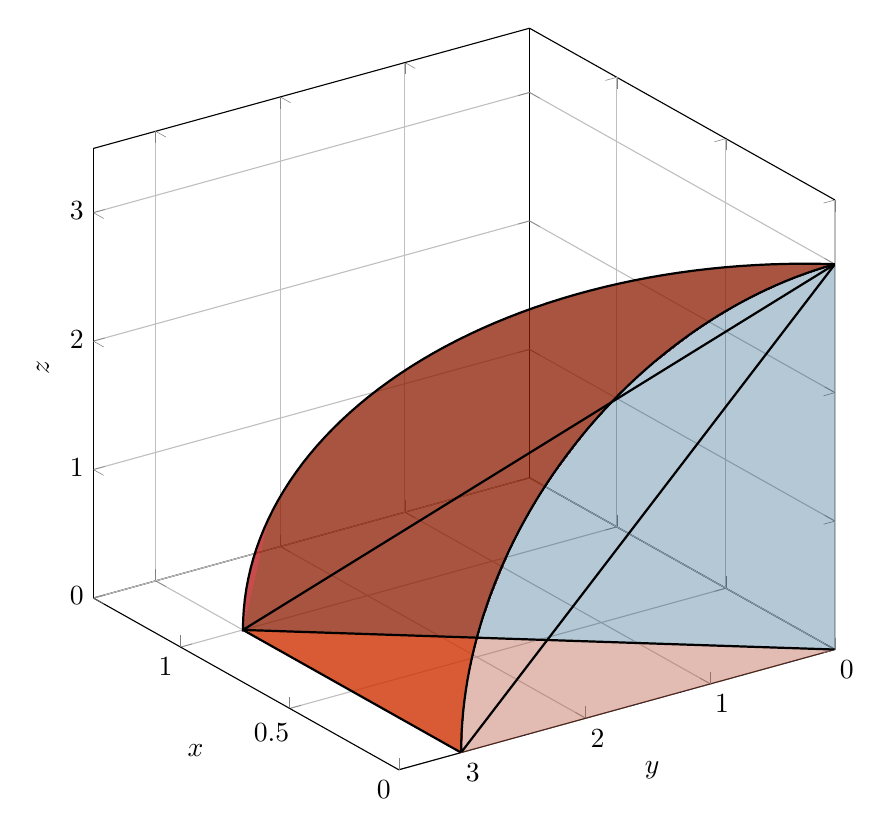
\begin{tikzpicture}
\begin{axis}[
    view={-125}{25},
    width=11cm, height=11cm,
    xlabel=$x$, ylabel=$y$, zlabel=$z$,
    xmin=0, xmax=1.4, ymin=0, ymax=3.5, zmin=0, zmax=3.5,
    trig format plots=deg,
    grid=major,
]
% curved roof : cylinder y^2+z^2=9, 0<=x<=y/3
\addplot3[surf, shader=interp, colormap={roof}{color=(red!70!black) color=(red!70!black)},
          opacity=0.70, domain=0:1, y domain=0:90, samples=10, samples y=25]
    ({x*cos(y)}, {3*cos(y)}, {3*sin(y)});
% face x = 0 (quarter disk)
\addplot3[surf, shader=interp, colormap={fblue}{color=(blue) color=(blue)},
          opacity=0.16, domain=0:3, y domain=0:90, samples=10, samples y=25]
    (0, {x*cos(y)}, {x*sin(y)});
% face y = 3x
\addplot3[surf, shader=interp, colormap={fgreen}{color=(green!50!black) color=(green!50!black)},
          opacity=0.16, domain=0:1, y domain=0:3, samples=10, samples y=25]
    ({y/3}, {y}, {x*sqrt(9-y^2)});
% bottom z = 0
\addplot3[surf, shader=interp, colormap={ffloor}{color=(orange) color=(orange)},
          opacity=0.30, domain=0:1, y domain=0:3, samples=10, samples y=25]
    ({x*y/3}, {y}, {0});
% --- bold edges of the roof ---
\addplot3[thick, black, domain=0:90, samples=60] (0, {3*cos(x)}, {3*sin(x)});
\addplot3[thick, black, domain=0:90, samples=60] ({cos(x)}, {3*cos(x)}, {3*sin(x)});
\addplot3[thick, black, domain=0:1, samples=10]  ({x}, {3}, {0});
\addplot3[thick, dashed, black, domain=0:1, samples=10] ({x}, {3*x}, {0});
\end{axis}
\end{tikzpicture}
\end{document}
